\documentclass[tikz, border=1mm]{standalone}

\usetikzlibrary{shapes}
\usetikzlibrary{patterns}

\begin{document}
	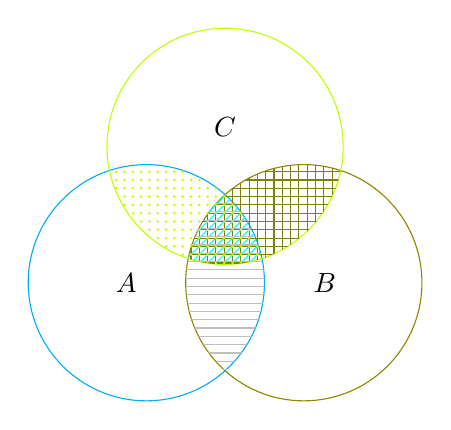
\begin{tikzpicture}
		\def\firstcircle{(0,0) circle (1.5 cm)}
		\def\secondcircle{(0: 2 cm) circle (1.5 cm)}
		\def\thirdcircle{(60:2 cm) circle (1.5 cm)}
		
		% Draw the circles
		\draw[color=cyan] \firstcircle;
		\draw[color=olive] \secondcircle;
		\draw[color=lime] \thirdcircle;
		
		% Fill the intersections
		\begin{scope}
			\clip \firstcircle;
			\clip \secondcircle;
			\fill[pattern=north east lines, pattern color=cyan] \thirdcircle;
		\end{scope}
		
		\begin{scope}
			\clip \secondcircle;
			\fill[pattern=grid, pattern color=olive] \thirdcircle;
		\end{scope}
		
		\begin{scope}
			\clip \firstcircle;
			\fill[pattern=dots, pattern color=lime] \thirdcircle;
		\end{scope}
		
		
		\begin{scope}
			\clip \firstcircle;
			\fill[pattern=horizontal lines, pattern color=lightgray] \secondcircle;
		\end{scope}
		
		% Label the sets
		\node[left] at (0,0) {$A$};
		\node[right] at (0:2 cm) {$B$};
		\node[above] at (60:2 cm) {$C$};
	\end{tikzpicture}
\end{document}

